\documentclass[12pt]{report}

\usepackage[norsk]{babel}
\usepackage{graphicx} % Required for inserting images
\usepackage{graphicx, array, carlito, fancyhdr, comment, etoc, lipsum, enumitem, standalone, subfiles, newclude, float, enumitem, amsmath, hyperref, adjustbox, titlesec, pdfpages}

\usepackage[style=ieee, sorting=none]{biblatex}

% Fjerne Teksten Kapittel fra overskrift. Justerer plasseringen av chapter navn
\titleformat{\chapter}[display]
{\Huge\bfseries}
{}
{-120pt}
{\thechapter.\ }
\titleformat{name=\chapter,numberless}[display]
{\Huge\bfseries}
{}
{-120pt}
{}
\titlespacing*{\chapter}{0pt}{70pt}{10pt} % Juster verdien 40pt for å endre avstanden


%Gir automatisk nytt avsnitt ved linjeskift
\usepackage[parfill]{parskip}

%Ikke inrykk ved nytt avsnitt
\setlength{\parindent}{0pt}

\usepackage{exsheets}
%Vis løsningsforslag på alle oppgaver
\SetupExSheets{solution/print=false}


\usepackage[a4paper, total={6in, 8in}]{geometry}



% Laste inn referanser
\addbibresource{backmatter/referanser.bib}

% Adding abstract funciton
\newcommand{\chapabstract}[1]{
	\begin{quote}
		\singlespacing\small
		\rule{14cm}{1pt}
		#1
		\vskip-4mm
		\rule{14cm}{1pt}
\end{quote}}


% Set up the fancyhdr package
\pagestyle{fancy}
\fancyhf{} % Clear all header and footer fields

% Adjust the footer position
\setlength{\footskip}{3cm} % You can adjust this value as needed

% Define the footer
%\fancyfoot[L]{\vspace{1cm} \makebox[0pt][l]{\hspace{0.5cm} Elektroniske systemer}} % Left-aligned course name, lifted up
\fancyfoot[R]{%
	\begin{minipage}{2cm}
		\centering
		
\includegraphics[height=1cm]{frontmatter/bilder/r171JViZ6gmf8WXujFQw.jpg}\\
%		\vspace{-0.5cm} % Adjust vertical space to center page number
%		\thepage
	\end{minipage}
}
%\fancyfoot[C]{\thepage}

\fancyhead{}
\fancyhead[LE,RO]{\nouppercase{\rightmark}}
\fancyhead[RE,LO]{Side \thepage}





% ------------------    HER STARTER DOKUMENTET   ------------------

\begin{document}
%Setter inn tittelsiden som eksternt dokument
\begin{titlepage}
    \begin{center}
    \vspace*{1cm}
    \Huge
    \textbf{Elektroniske systemer}
    
    \LARGE
    \vspace{0.5cm}
    Øvingsoppgaver for analoge komponenter og måleteknikk i emnet elektroniske systemer

    \vspace{1.5cm}
    \textbf{Carl Magnus Bøe}
    
    2025

\vfill




    
\includegraphics[width=0.6\textwidth]{frontmatter/bilder/r171JViZ6gmf8WXujFQw.jpg}
    \Large
    
    Fagskolen Viken\\
    01TE00F EITKELFH24\\
    Fredrikstad\\

    \end{center}
\end{titlepage}

%Innholdsfortegnelse
\tableofcontents
\chapter{Introduksjon}
\label{ch:introduksjon}
Dette kapittelet inneholder generell informasjon om kompendiet med bakgrunn for arbeidet, oppbygging av dokumentet og lisensinformasjon.

\section{Bakgrunnsinformasjon}
Dette dokumentet er et kompendium som inneholder øvingsoppgaver relevante for delen analoge komponenter i emnet elektroniske systemer. Siden dokumentet blir kontinuerlig revidert, er det datomerkingen på forsiden som angir versjonen av dokumentet. Målet med dette dokumentet er å samle alle øvingsoppgaver sammen med løsningsforslagene i ett dokument.

Når man jobber med oppgavene, anbefales det at man også gjør simuleringer. %Noen anbefalte simuleringsverktøy er omtalt i Kapittel \ref{ch:programvare}.

Dersom du har kommentarer, forslag til oppgaver eller har funnet noe som er feil, vennligst send en epost til \href{mailto:carlbo@afk.no}{carlbo@afk.no}.

\section{Oppbygning av kompendiet}
Kompendiet er delt opp i hovedgrupper, hvor undergrupper som forskjellige elektroniske komponenter er beskrevet som seksjoner. For hver seksjon presenteres først alle oppgavene, før løsningsforslaget blir presentert i neste seksjon.

\begin{comment}
	\section{Lisensinformasjon}
	Dette dokumentet er basert på materiale fra \textit{Lessons In Electric Circuits} av Tony R. Kuphaldt, distribuert under Design Science License. Originaldokumentet kan finnes på \href{https://www.ibiblio.org/kuphaldt/electricCircuits/}{Lessons In Electric Circuits}. Eventuelle modifikasjoner og avledede verk er også distribuert under Design Science License.
	
	Deler av dette kompendiet er utviklet av Carl Magnus Bøe. Disse delene inkluderer:
	\begin{enumerate}[label=\roman*)]
		\item Kapittel \ref{sec:diodeOppgave} / \ref{sec:diodeLøsning}
		\item 
	\end{enumerate}
\end{comment}
\chapter{Programvare}
\label{ch:programvare}
Dette kapittelet omtaler forskjellig programvare relevant i emnet.


\section{Simulering}
\subsection{CircuitMaker2000}
\href{https://winworldpc.com/product/circuitmaker/2000}{CircuitMaker2000}
\subsection{LTspice}
\href{https://www.analog.com/en/resources/design-tools-and-calculators/ltspice-simulator.html}{LTspice}
\subsection{OpenModelica}
\href{https://openmodelica.org/}{OpenModelica}

\section{Tegne kretser}
\subsection{Draw.io}


\chapter{Analoge komponenter}

\section{Dioder}


Dette kapittelet inneholder oppgaver relatert til halvleder dioder. Om ingenting annet er gitt i oppgaven så antar vi et ideelt spenningsfall over dioden på $0,7[V]$.\\
\subsection{Lysdioder - LED}
Lysdioder har forskjellige spenningsfall for samme farge avhengig av modellserie og produsent. For optimal verdi må man lese databladet til dioden. 

Tabell \ref{tab:LEDspenningsfall} viser et generelt spenn av verdier.

\begin{table}[!ht]
	\caption{Spenningsfall for forskjellige lysdioder}
	\label{tab:LEDspenningsfall}
	\begin{center}
		\begin{tabular}{|l|c|c|} 
			\hline
			Farge & Spenningsfall & Enhet \\ [0.5ex] 
			\hline\hline
			Hvit & $3,0 - 5,0$ &$ [V]$ \\
			\hline
			Fiolett: &  $2,8 - 4,0$ &$ [V]$\\
			\hline
			Blå: &  $2,5 - 3,7$ &$ [V]$\\
			\hline
			Grønn: &  $1,6 - 4,0$ &$ [V]$\\
			\hline
			Gul: &  $2,0 - 2,4$ &$ [V]$\\
			\hline
			Oransje: &  $2,0 - 2,1$ &$ [V]$\\
			\hline
			Rød: &  $1,5 - 2,0$ &$ [V]$\\
			\hline
			Infrarød: &  $1,2 - 1,9$ &$ [V]$\\
			\hline
		\end{tabular}
	\end{center}
\end{table}



%Setter inn oppgaver fra ekstern ark
\subsection{Oppgaver}
\subsubsection{Dioder}
\input{diode/oppgaver_dioder}
\subsubsection{Zenerdioder}
\input{diode/oppgaver_zenerdioder}

\subsection{Løsningsforslag}
\printsolutions[section]



\newpage

\section{Tyristor, triac og diac}
\begin{question}[name=Spørsmål, topic=tyristor]
	Tegn symbolene for følgende komponenter.
	\begin{enumerate}[label=\roman*]
		\item Halvlederdiode
		\item LED
		\item Zenerdiode
	\end{enumerate}
\end{question}


\begin{solution}[name=Løsningsforslag]
tatata

%	\begin{figure}[H]
%		\centering
%		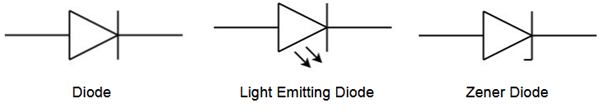
\includegraphics[width=0.7\textwidth]{diode/figurer/oppgave1.png}
%		\caption{Eksempel på forskjellige diode symboler.}
%		\label{fig:diodeSeeeymb}
%	\end{figure}
\end{solution}
\printsolutions[section]

\section{BJT transisor}

\section{FET transistor}

\section{Forsterker i praksiss}

\section{Måleteknikk}

\newpage

\printbibliography%[title={Referanser}]

\appendix
\chapter[LED Datasheet]{LED Datasheet}
\label{paper-a}

\emph{Datablad fra en standard LED \cite{LEDdatasheet}.}
	
	\bigskip

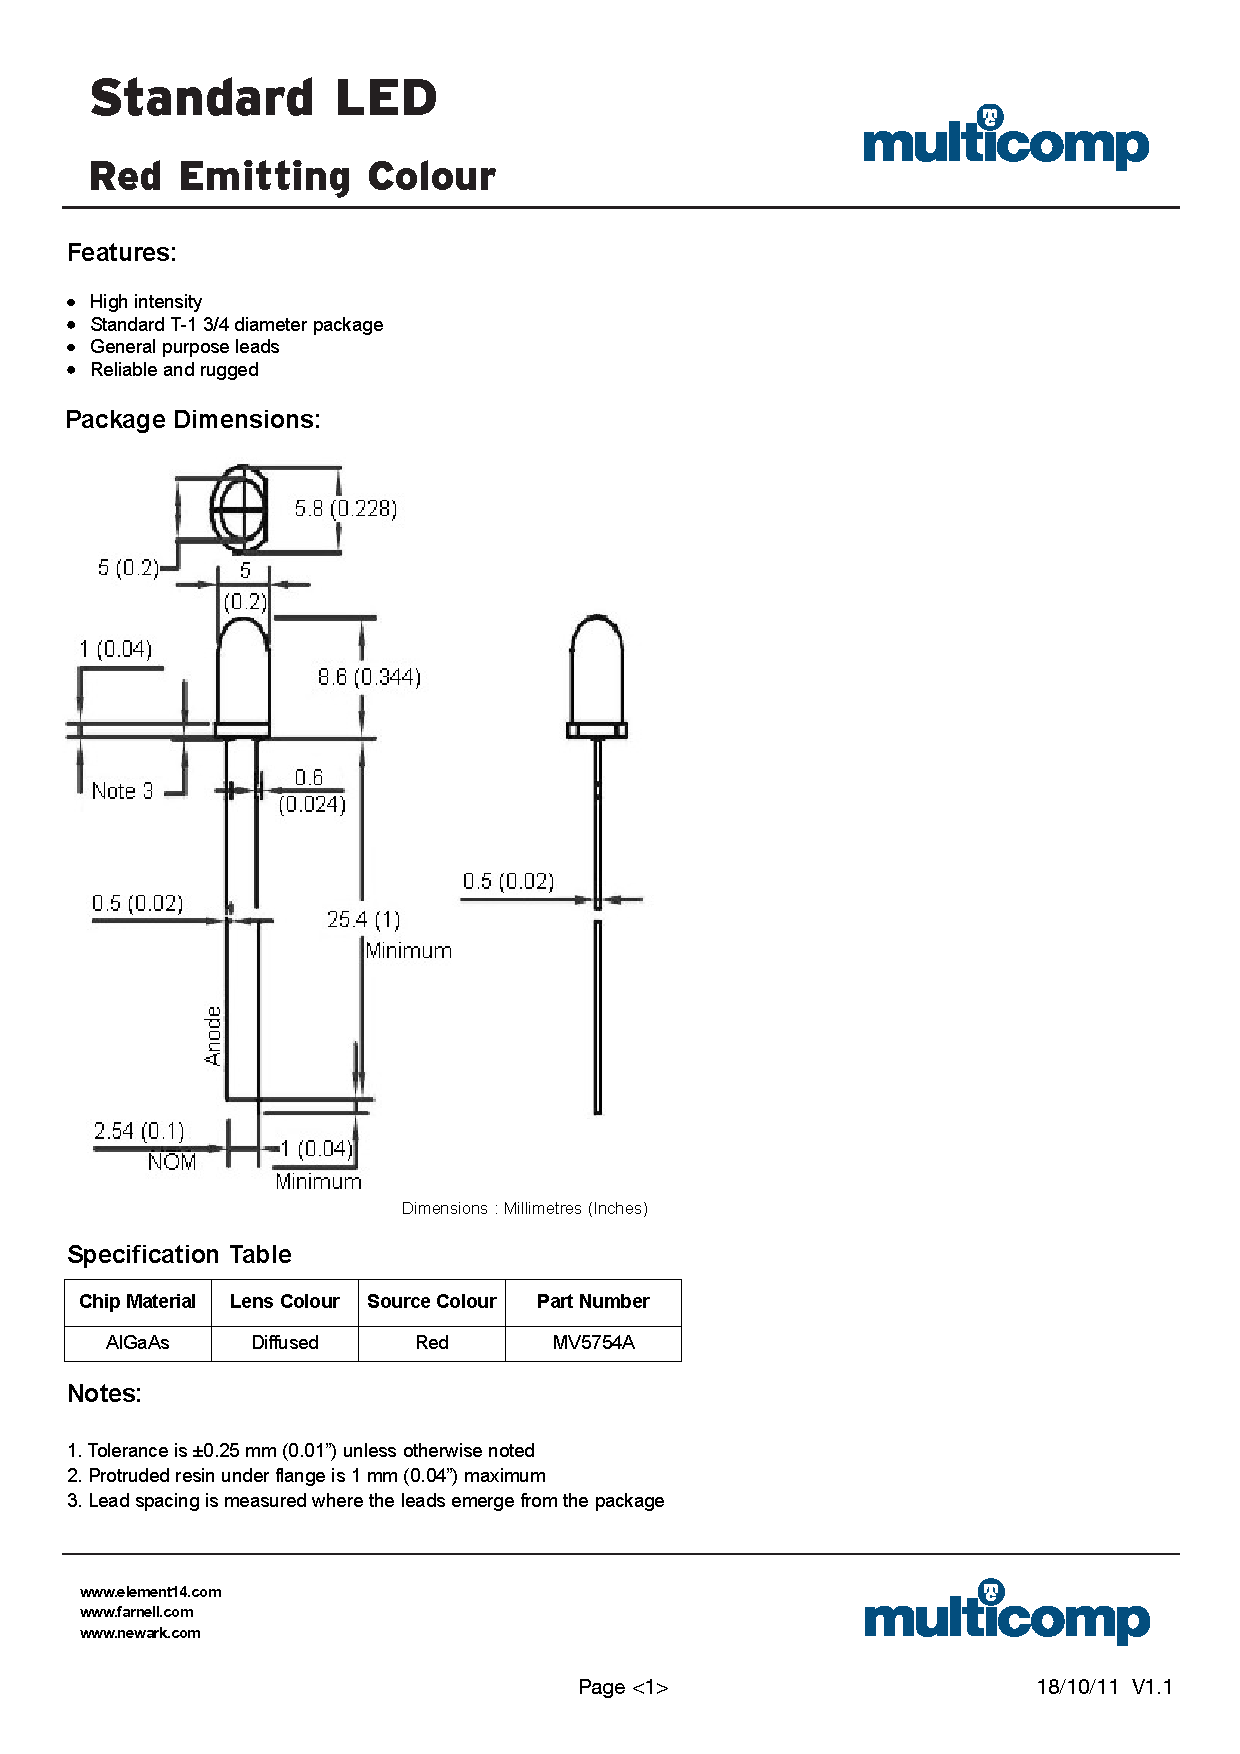
\includepdf[pages=-]{backmatter/pdfVedlegg/1LED_datasheet1498852.pdf}


\end{document}
